\chapter{Слежение для системы с астатизмом первого порядка (И-регулятор)}
\label{ch:chap4}

Теперь будем работать с интегральным регулятором следующего вида:
$$
H(s) = \frac{k}{s}
$$


\section{Стационарный режим работы}
Будем пытаться угнаться за сигналом $g(t) = A = 2$.
Выберем следующие $k$:
$$
k_1 = 0.05, k_2 = 0.5,  k_3 = 0.3
$$

Аналитически определим $e_{final}$ пользуясь теоремой о предельном значении для каждого $k$:
$$
\lim_{t\to\infty} y(t) = \lim_{s\to 0}sE(s)
$$
Для начала найдём образ ошибки слежения: $E(s) = W_{g\to e}(s)G(s)$
$$
W_{g\to e} = \frac{1}{1+W(s)} = \frac{s(s^2 +2.5s + 1)}{s(s^2 + 2.5s + 1) + 3k}
$$
$$
G(s) = \frac{A}{s}
$$
$$
E(s) = \frac{A(s^2 +2.5s + 1)}{s(s^2 + 2.5s + 1) + 3k}
$$
В итоге:
$$
\begin{aligned}
  \lim_{t\to\infty} y(t) = \lim_{s\to 0}s\frac{As^2(s^2 +2.5s + 1)}{s(s^2 + 2.5s + 3k + 1)} = 0\\
\end{aligned}
$$
А это значит, что наш астатизм справился с постоянным сигналом, успеваем.

\begin{figure}[ht]
  \centering
  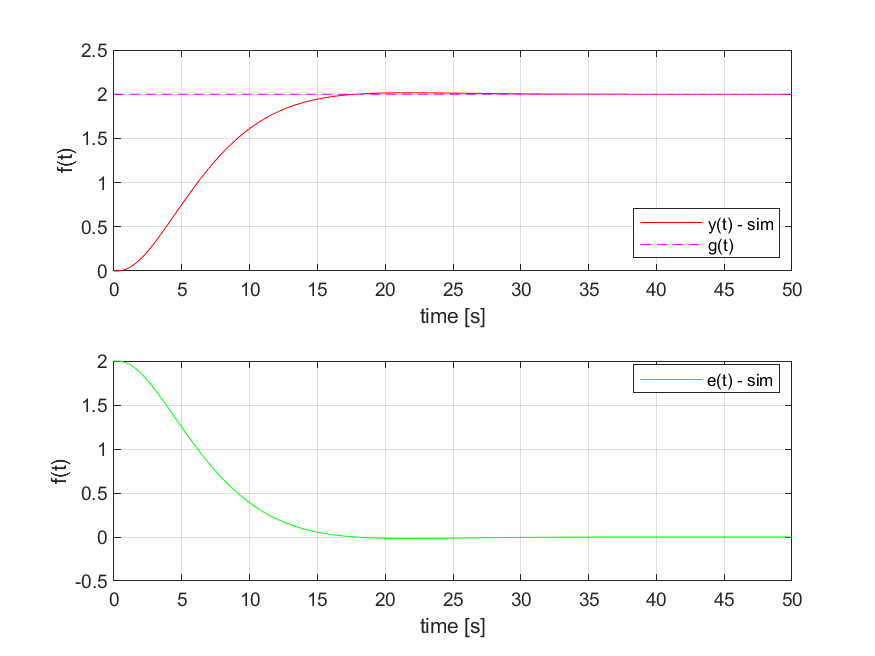
\includegraphics[width=0.8\textwidth]{output_task4_exp1.png}
\caption{Симуляция - стационарный, $k=0.05$}
\end{figure}

\newpage
\begin{figure}[ht]
  \centering
  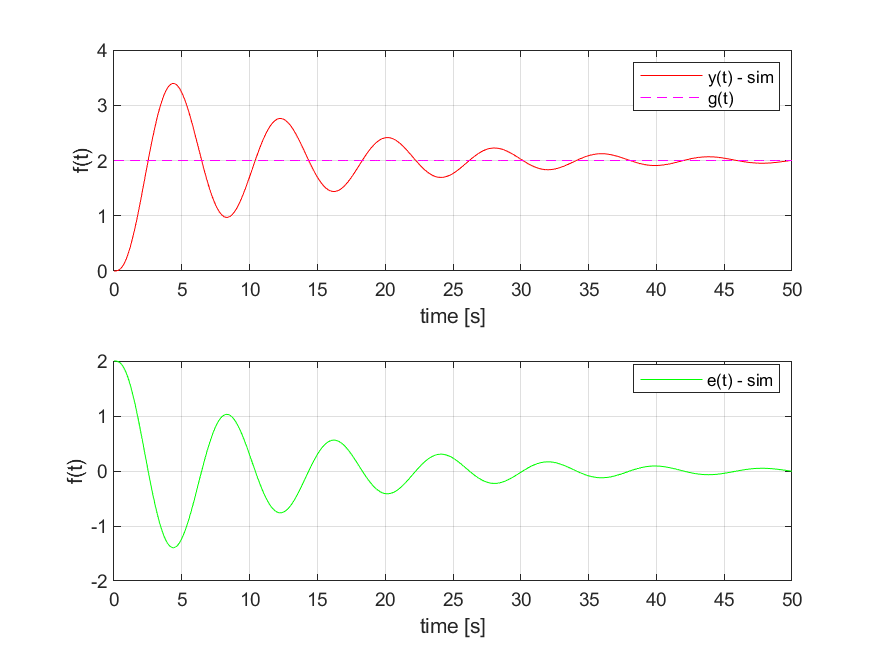
\includegraphics[width=0.8\textwidth]{output_task4_exp2.png}
\caption{Симуляция - стационарный, $k=0.5$}
\end{figure}

\begin{figure}[ht]
  \centering
  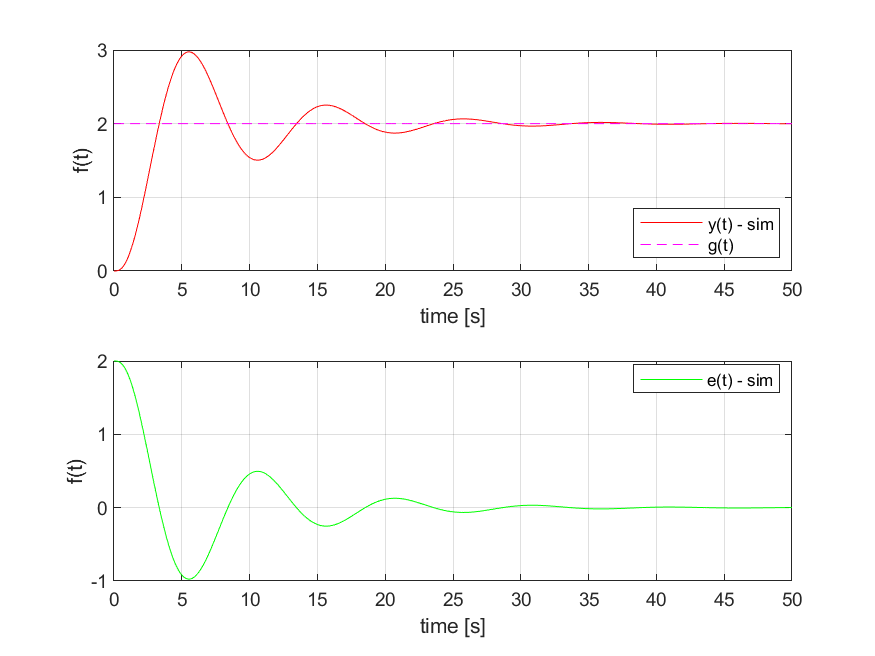
\includegraphics[width=0.8\textwidth]{output_task4_exp3.png}
\caption{Симуляция - стационарный, $k=0.3$}
\end{figure}

\newpage
\begin{figure}[ht]
  \centering
  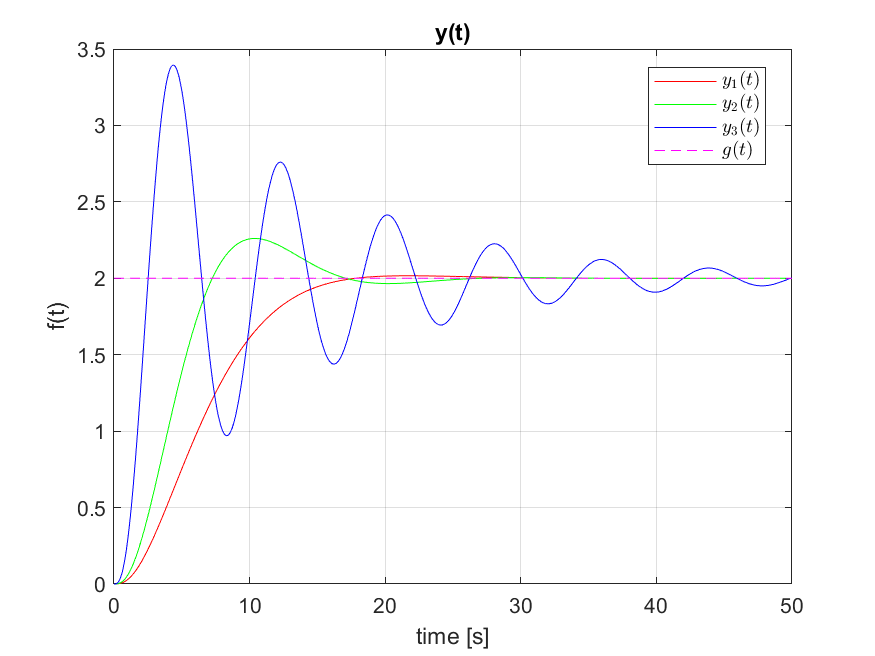
\includegraphics[width=0.8\textwidth]{output_task4_exp4.png}
\caption{Симуляция - стационарный, сравнение сигналов}
\end{figure}

\begin{figure}[ht]
  \centering
  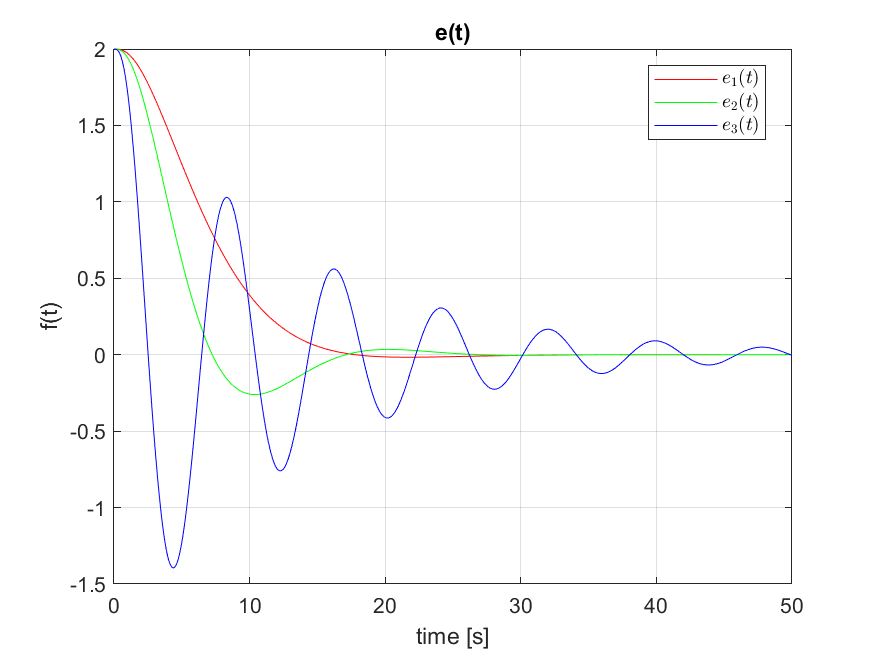
\includegraphics[width=0.8\textwidth]{output_task4_exp5.png}
\caption{Симуляция - стационарный, сравнение ошибок}
\end{figure}

\newpage
\textbf{Выводы:} при увеличении $k$ начальная амплитуда сигнала $y(t)$ будет больше, а также увеличится время переходного процесса, но рано или поздно мы придём(полностью совпадать) к $g(t)$. 
При небольших $k$ мы приходим к цели быстрее и с мягкими колебаниями.

\section{Движение с постоянной скоростью}
Будем пытаться угнаться за сигналом $g(t) = Vt = 2t$ в случае моего варианта.
Выберем следующие $k$:
$$
k_1 = 0.5, k_2 = 0.05,  k_3 = 0.1
$$

Аналитически определим $e_{final}$ пользуясь теоремой о предельном значении:
$$
W_{g\to e} = \frac{1}{1+W(s)} = \frac{s(s^2 +2.5s + 1)}{s(s^2 + 2.5s + 1) + 3k}
$$
$$
G(s) = \frac{V}{s^2}
$$
Образ ошибки слежения:
$$
E(s) = \frac{Vs(s^2 +2.5s + 1)}{s^2(s(s^2 + 2.5s + 1) + 3k)}
$$
В итоге:
$$
\begin{aligned}
  \lim_{t\to\infty} y(t) = \lim_{s\to 0}s\frac{Vs^2(s^2 +2.5s + 1)}{s^2(s(s^2 + 2.5s + 1) + 3k)} =  \\
  \lim_{t\to\infty} y(t) = \lim_{s\to 0}s\frac{V(s^2 +2.5s + 1)}{s(s^2 + 2.5s + 1) + 3k)} =  \frac{V}{3k} =  \frac{2}{3k}
\end{aligned}
$$
Посчитаем ошибки для каждого $k$:
$$
\begin{aligned}
  e_1 = 4/3 \\
  e_2 = 40/3\\
  e_3 = 20/3
\end{aligned}
$$

\begin{figure}[ht]
  \centering
  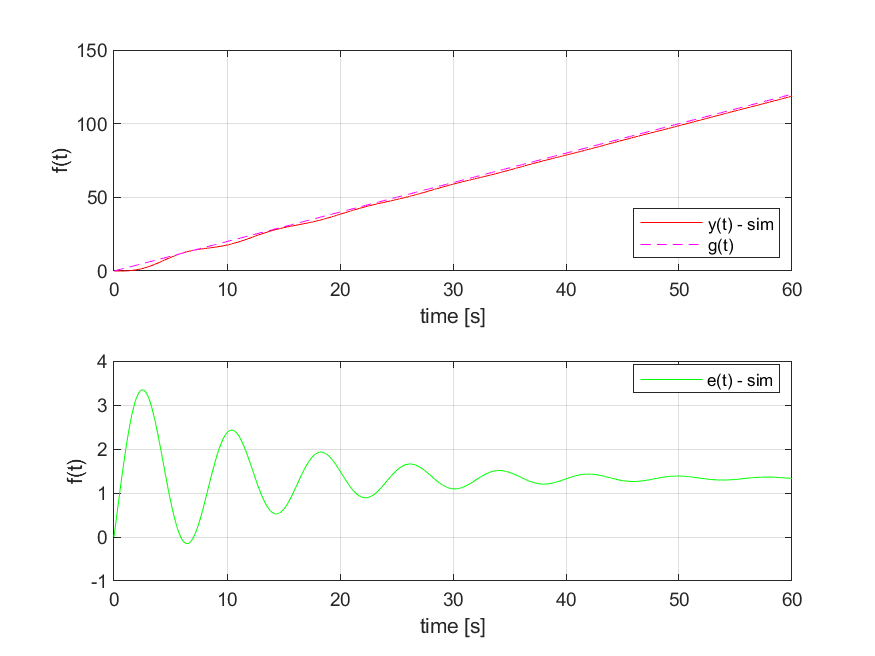
\includegraphics[width=0.8\textwidth]{output_task4_exp6.png}
\caption{Симуляция - постоянная скорость, $k=0.5$}
\end{figure}

\newpage
\begin{figure}[ht]
  \centering
  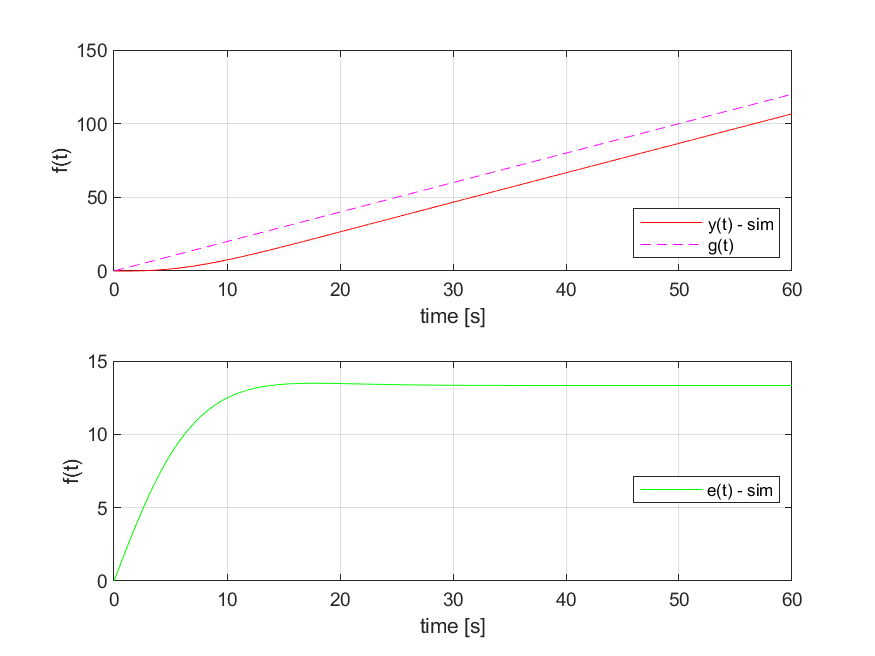
\includegraphics[width=0.8\textwidth]{output_task4_exp7.png}
\caption{Симуляция - постоянная скорость, $k=0.05$}
\end{figure}

\begin{figure}[ht]
  \centering
  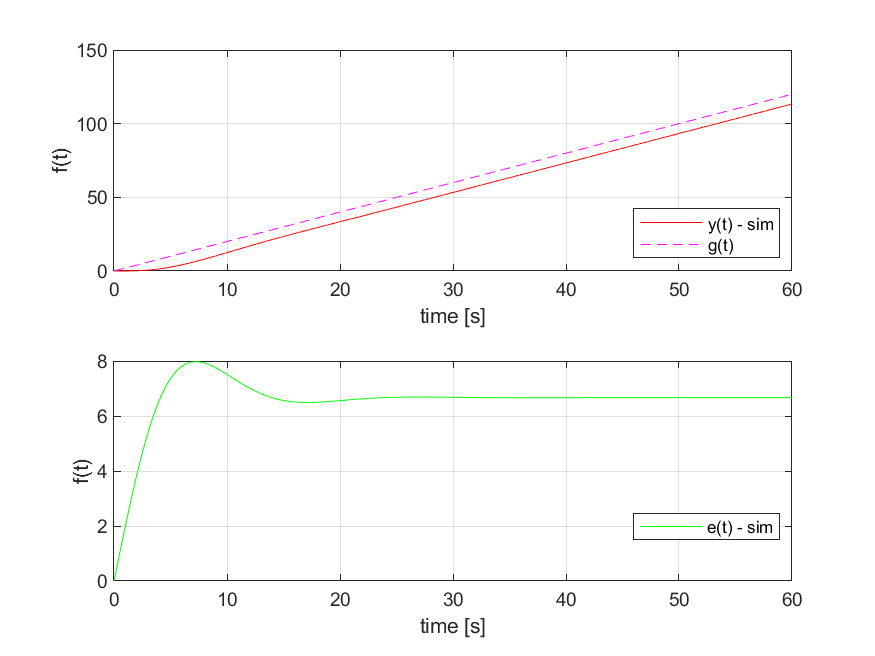
\includegraphics[width=0.8\textwidth]{output_task4_exp8.png}
\caption{Симуляция - постоянная скорость, $k=0.1$}
\end{figure}

\newpage
\begin{figure}[ht]
  \centering
  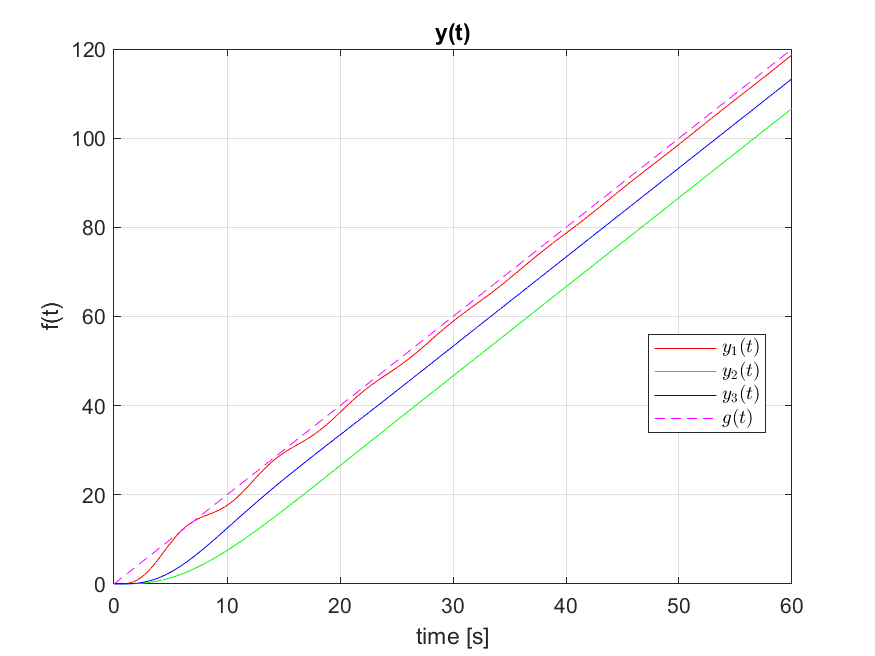
\includegraphics[width=0.8\textwidth]{output_task4_exp9.png}
\caption{Симуляция - постоянная скорость, сравнение сигналов}
\end{figure}

\begin{figure}[ht]
  \centering
  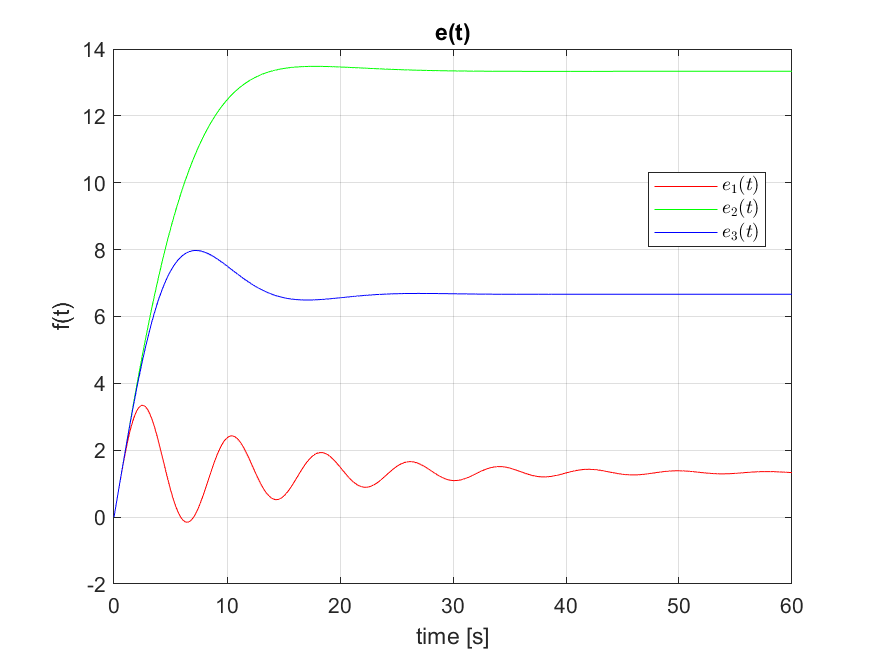
\includegraphics[width=0.8\textwidth]{output_task4_exp10.png}
\caption{Симуляция - постоянная скорость, сравнение ошибок}
\end{figure}

\newpage
\textbf{Выводы:} Так как система имеет у нас астатизм первого порядка, то и линейный сигнал она должна "почти" догонять, с точностью до установившейся ошибки,
что тоже неплохо, в нашем случае $e_{final} = \frac{2}{3k}$. 

Как можно заметить по общему графику ошибок - чем больше $k$, тем $y(t)$ ближе к $g(t)$, и также больше колебаний. И наоборот - чем меньше $k$, тем мы дальше будет от $g(t)$, но с куда меньшими колебаниями.


\section{Движение с постоянным ускорением}

Будем пытаться угнаться за сигналом $g(t) = \frac{at^2}{2} = 0.5t^2 = Bt^2$ в случае моего варианта.

Выберем следующие $k$:
$$
k_1 = 0.05, k_2 = 0.1,  k_3 = 0.5
$$

Определим установившуюся ошибку, пользуясь теоремой о предельном значении:
$$
W_{g\to e} = \frac{1}{1+W(s)} = \frac{s(s^2 +2.5s + 1)}{s(s^2 + 2.5s + 1) + 3k}
$$
$$
G(s) = \frac{2B}{s^3}
$$
Образ ошибки слежения:
$$
E(s) = \frac{2Bs(s^2 +2.5s + 1)}{s^2(s(s^2 + 2.5s + 1) + 3k)}
$$
В итоге:
$$
\begin{aligned}
  \lim_{t\to\infty} y(t) = \lim_{s\to 0}s\frac{2Bs^2(s^2 +2.5s + 1)}{s^3(s(s^2 + 2.5s + 1) + 3k)} =  \\
  = \lim_{s\to 0}s\frac{2B(s^2 +2.5s + 1)}{s(s(s^2 + 2.5s + 1) + 3k))} = \frac{2B}{0} = \infty
\end{aligned}
$$

А значит при любом $k$ ошибка будет улетать в бесконечность.. сигналы $y(t)$ и $g(t)$ будут расходиться

\begin{figure}[ht]
  \centering
  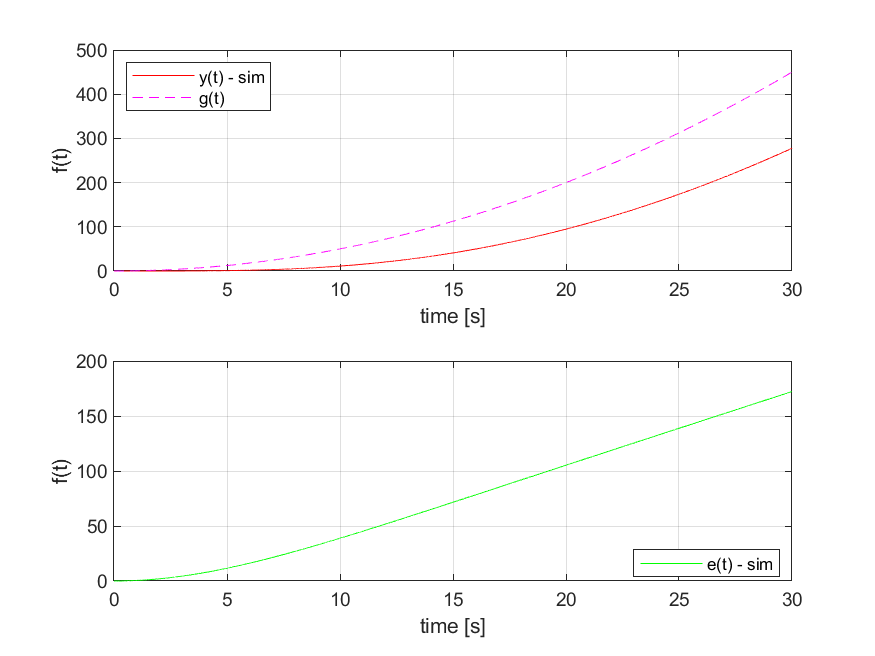
\includegraphics[width=0.8\textwidth]{output_task4_exp11.png}
\caption{Симуляция - постоянное ускорение, $k=0.05$}
\end{figure}

\newpage
\begin{figure}[ht]
  \centering
  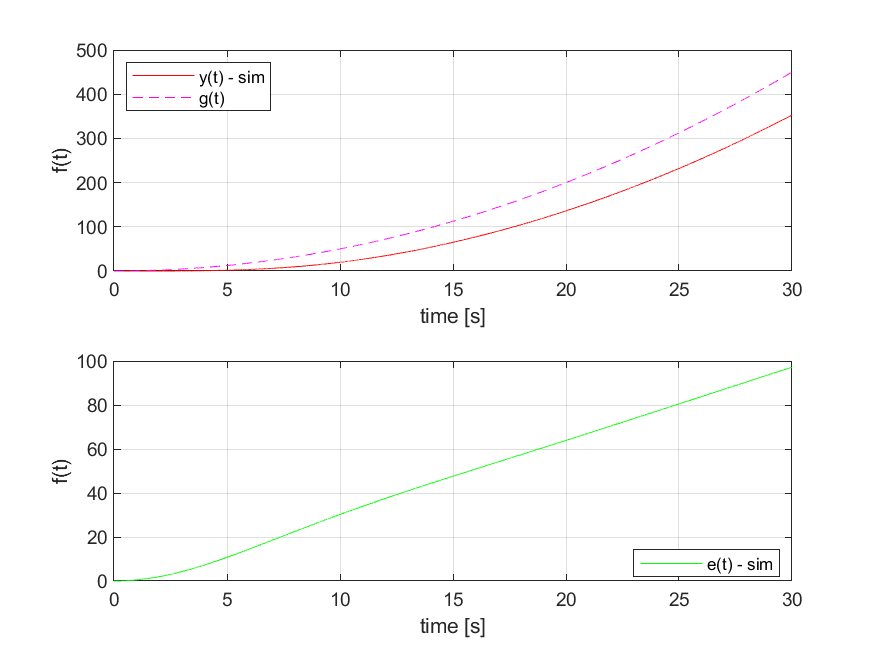
\includegraphics[width=0.8\textwidth]{output_task4_exp12.png}
\caption{Симуляция - постоянное ускорение, $k=0.1$}
\end{figure}

\begin{figure}[ht]
  \centering
  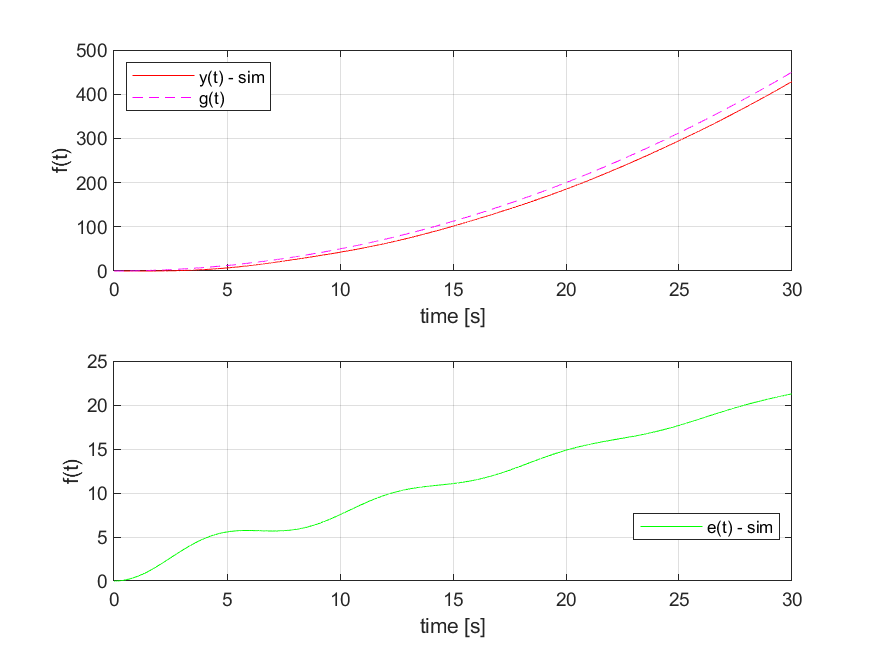
\includegraphics[width=0.8\textwidth]{output_task4_exp13.png}
\caption{Симуляция - постоянное ускорение, $k=0.5$}
\end{figure}

\newpage
\begin{figure}[ht]
  \centering
  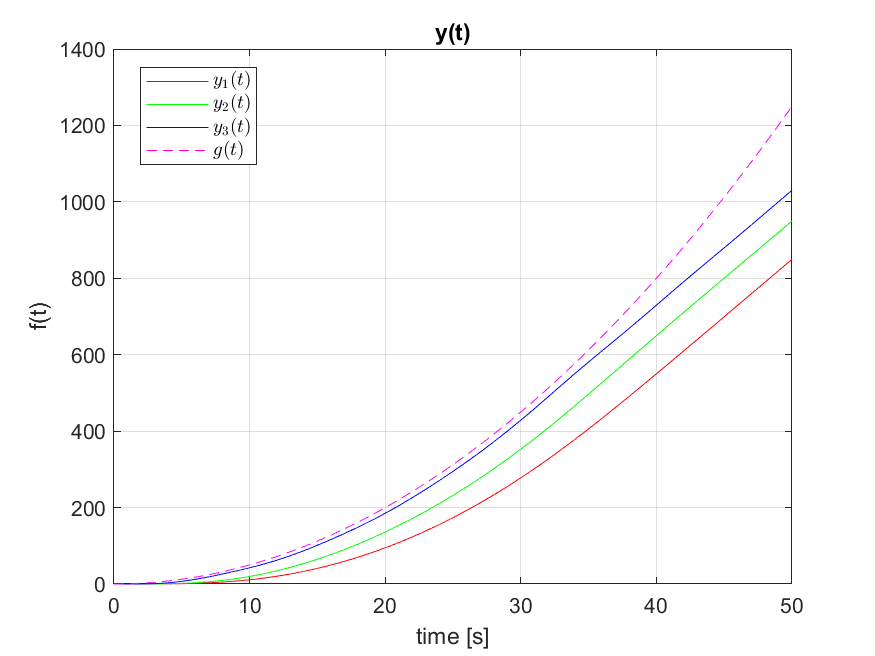
\includegraphics[width=0.8\textwidth]{output_task4_exp14.png}
\caption{Симуляция - постоянное ускорение, сравнение сигналов}
\end{figure}

\begin{figure}[ht]
  \centering
  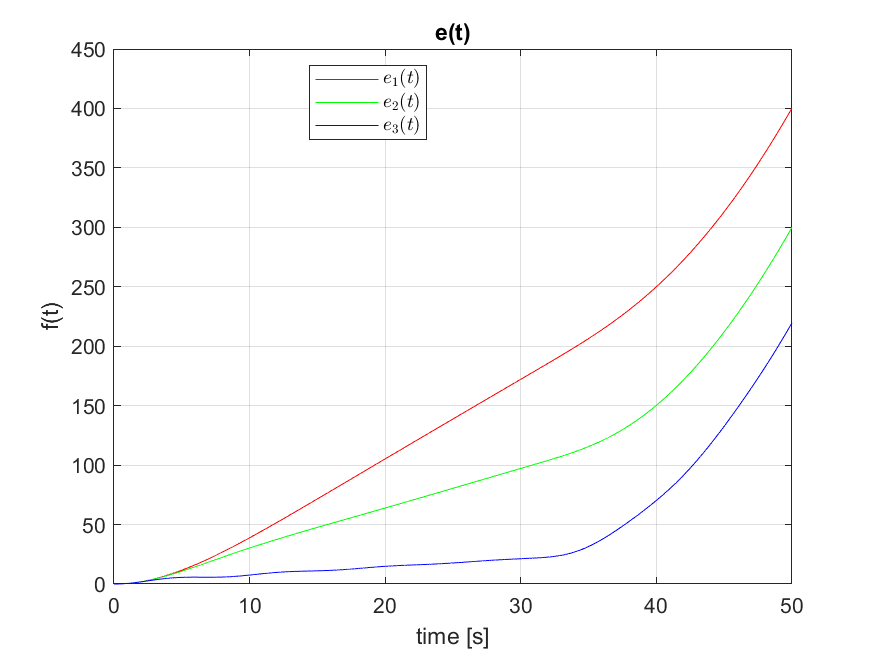
\includegraphics[width=0.8\textwidth]{output_task4_exp15.png}
\caption{Симуляция - постоянное ускорение, сравнение ошибок}
\end{figure}

\newpage
\textbf{Выводы:} сигналы будут расходиться, но при этом график ошибки возрастает линейно, и чем больше у нас $k$, тем плавнее и дольше будет происходить отдаление на бесконечность (и наоборот).

\endinput